\chapter{Conference and Local Information}

\setlength\fboxsep{0pt}
\setlength\fboxrule{0.5pt}
%\phantomsection \section{Help and Emergencies}

%In case of an emergency at the conference, please call {\Large \textbf{911}}. You can also request help from any of the conference volunteers and the concierge at the main entrances of university buildings. For emergencies at the conference or elsewhere in USA, please call the emergency number {\Large \textbf{911}}. 

%If you need special assistance to access a building, please contact the registration desk at {\Large \textbf{NUMBER}}.

\phantomsection \section{About University of California, Berkeley}

The University of California, Berkeley (also referred to as UC Berkeley; Berkeley; California; or simply Cal), is a public research university located in Berkeley, California. The university occupies 1,232 acres (499 ha) on the eastern side of the San Francisco Bay with the central campus resting on 178 acres (72 ha). Berkeley is the flagship institution of the 10 campus University of California system.

Established in 1868 as the result of the merger of the private College of California and the public Agricultural, Mining, and Mechanical Arts College in Oakland, Berkeley is the oldest institution in the UC system and offers approximately 350 undergraduate and graduate degree programs in a wide range of disciplines. Berkeley has been charged with providing both "classical" and "practical" education for the state's people. Berkeley co-manages three United States Department of Energy National Laboratories, including the Los Alamos National Laboratory, Lawrence Livermore National Laboratory and Lawrence Berkeley National Laboratory for the U.S. Department of Energy.

Berkeley faculty, alumni, and researchers have won 72 Nobel Prizes (including 30 alumni Nobel laureates), 9 Wolf Prizes, 7 Fields Medals, 15 Turing Awards, 45 MacArthur Fellowships, 20 Academy Awards, and 11 Pulitzer Prizes. To date, UC Berkeley scientists have discovered 6 chemical elements of the periodic table (californium, seaborgium, berkelium, einsteinium, fermium, lawrencium). Along with Berkeley Lab, UC Berkeley researchers have discovered 16 chemical elements in total – more than any other university in the world. Berkeley is a founding member of the Association of American Universities and continues to have very high research activity with \$652.4 million in research and development expenditures in 2009. Berkeley physicist J. Robert Oppenheimer was the scientific director of the Manhattan Project that developed the first atomic bomb in the world, which he personally headquartered at Los Alamos, New Mexico, during World War II. Faculty member Edward Teller was (together with Stanislaw Ulam) the "father of the hydrogen bomb". Former United States Secretary of Energy and Nobel laureate Steven Chu (PhD 1976), was Director of Berkeley Lab from 2004-2009.

\vspace{1cm}
\phantomsection
\section{Internet / Wireless LAN}

%TODO tell people to look up the USB stick for information on how to configure, and contact registration desk in case of troubles
Conference participants will be able to access the campus-wide wireless \emph{AirBears} network. Access credentials are printed on your name tag. If you have difficulties setting up your wireless, please contact any of the volunteers or the registration desk.



\clearpage
\phantomsection \section{Conference and Workshops Venues:}
%The following campus map shows the location.
\begin{figure}[h!]
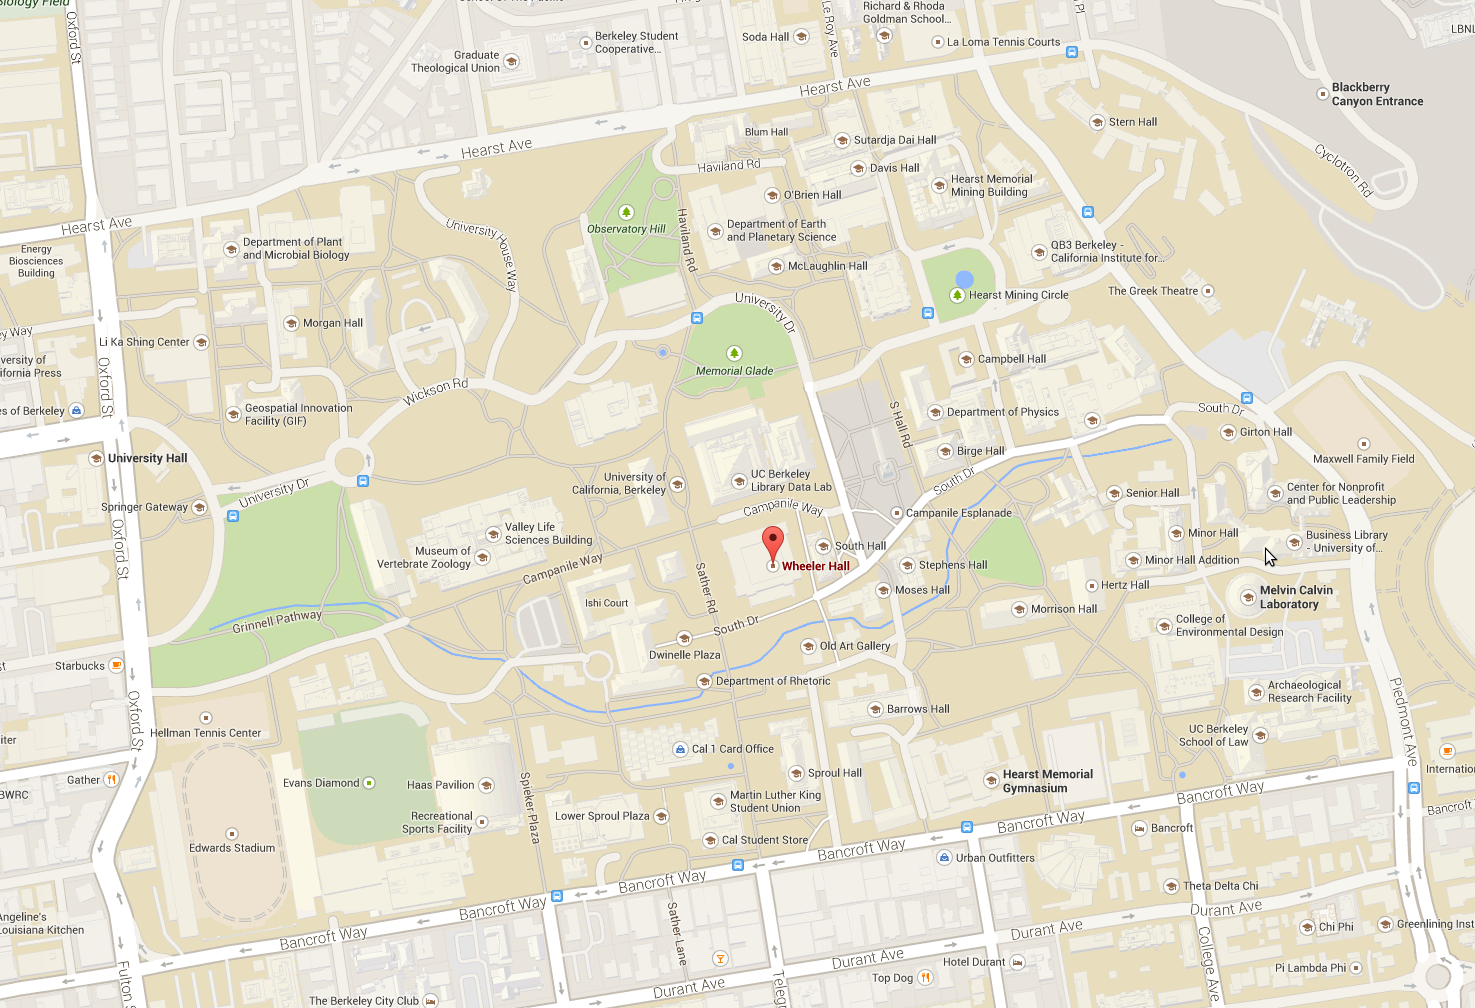
\includegraphics[width=\linewidth]{local_img/maps/wheeler_hall}
\end{figure}

The conference, the workshops and interactive poster sessions will take place in the Wheeler Hall of UC Berkeley. 

\newpage
\phantomsection \section{1st Floor Plan of Wheeler Hall -- Conference Venue}
{\large Monday, July 14 to Wednesday, July 16}
\begin{figure}[h!]
\center
\includegraphics[height=0.6\textheight]{local_img/maps/first_floor}
\end{figure}

\newpage
\phantomsection \section{2nd Floor plan of Wheeler Hall -- Workshops Venue}
{\large Saturday, July 12 to Sunday, July 13}

\begin{figure}[h!]
\center
\includegraphics[height=0.6\textheight]{local_img/maps/second_floor}
\end{figure}

\vspace{1.0cm}
{On Saturday, July 12, on-site registration will be held on the first floor of Wheeler Hall}

\clearpage

\phantomsection \section{Floor Plan Interactive Presentations}

The numbers indicate monitors for the interactive paper presentations. Please refer to the conference program to find the right monitor for each paper.
\begin{figure}[h!]
\center
\includegraphics[height=0.6\textheight]{local_img/maps/basement}
\end{figure}



\phantomsection \section{Banquet Information}
The conference banquet will be held on a cruise on the San Francisco Bay. Enjoy a splendid sunset on the water with magnificent views of the city of San Francisco, accompanied by a
delicious seasonal dinner and drinks. Transportation will be provided. Buses will pick us up from Berkeley at 6pm and take us to Pier 3 in San Francisco, where we will board the San Francisco Belle. Buses will pick us up from Pier 3 around 10pm, and we'll be back in Berkeley
around 10:30pm.

%\label{sec:banquetinfo}
%\begin{figure}[h!]
%\center
%\fbox{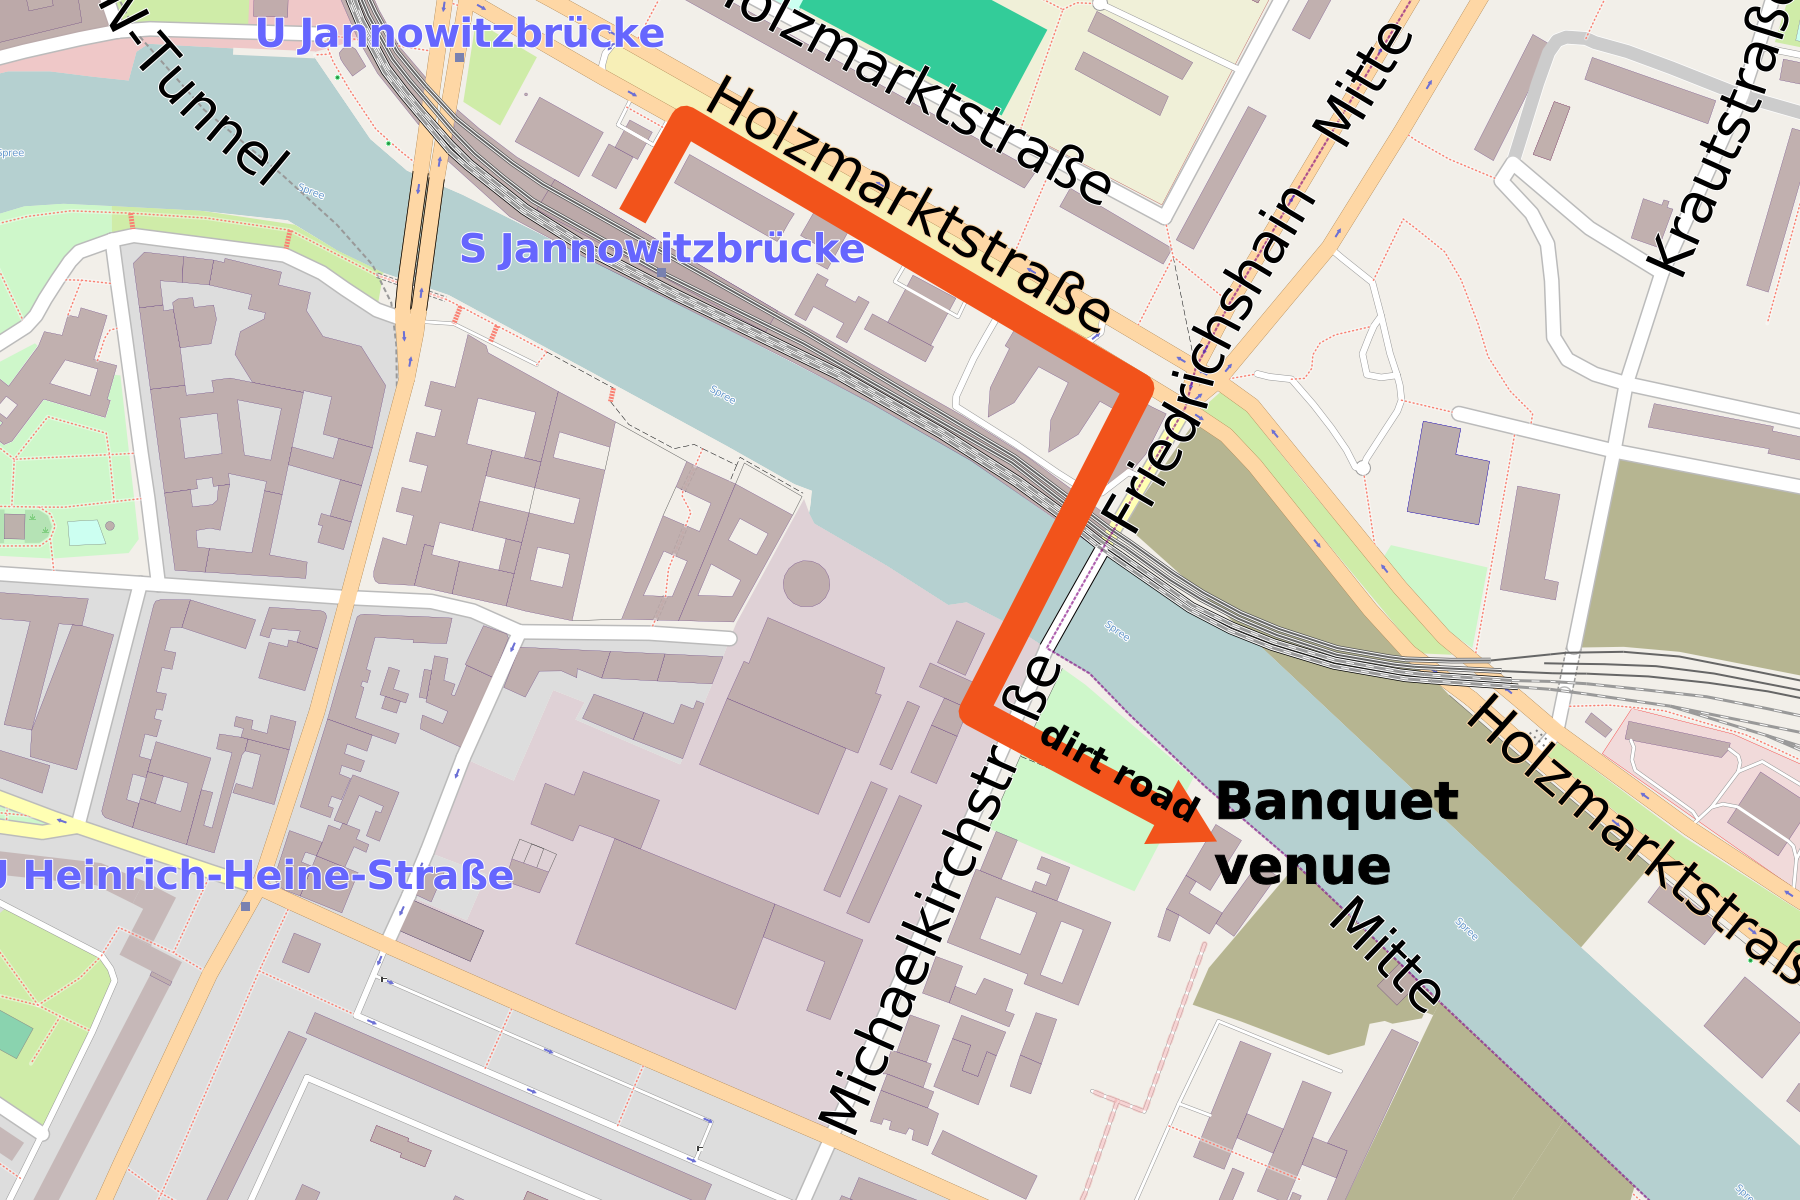
\includegraphics[width=3in]{local_img/maps/katerholzig_labeled}}
%\end{figure}

%After crossing the bridge, turn left through a boarded fence and enter the venue via an unpaved path. When you start wondering whether you are at the right place, you are at the right place.  Just keep on walking.  The address of Kater Holzig is Michaelkirchstra{\ss}e 23; the GPS coordinates are: 52.511283,13.42393. 

%The trip takes about 45 minutes. The banquet will begin at 20:00.


%\begin{landscape}
%\phantomsection \section{Public transport map}
%\begin{figure}[h!]
%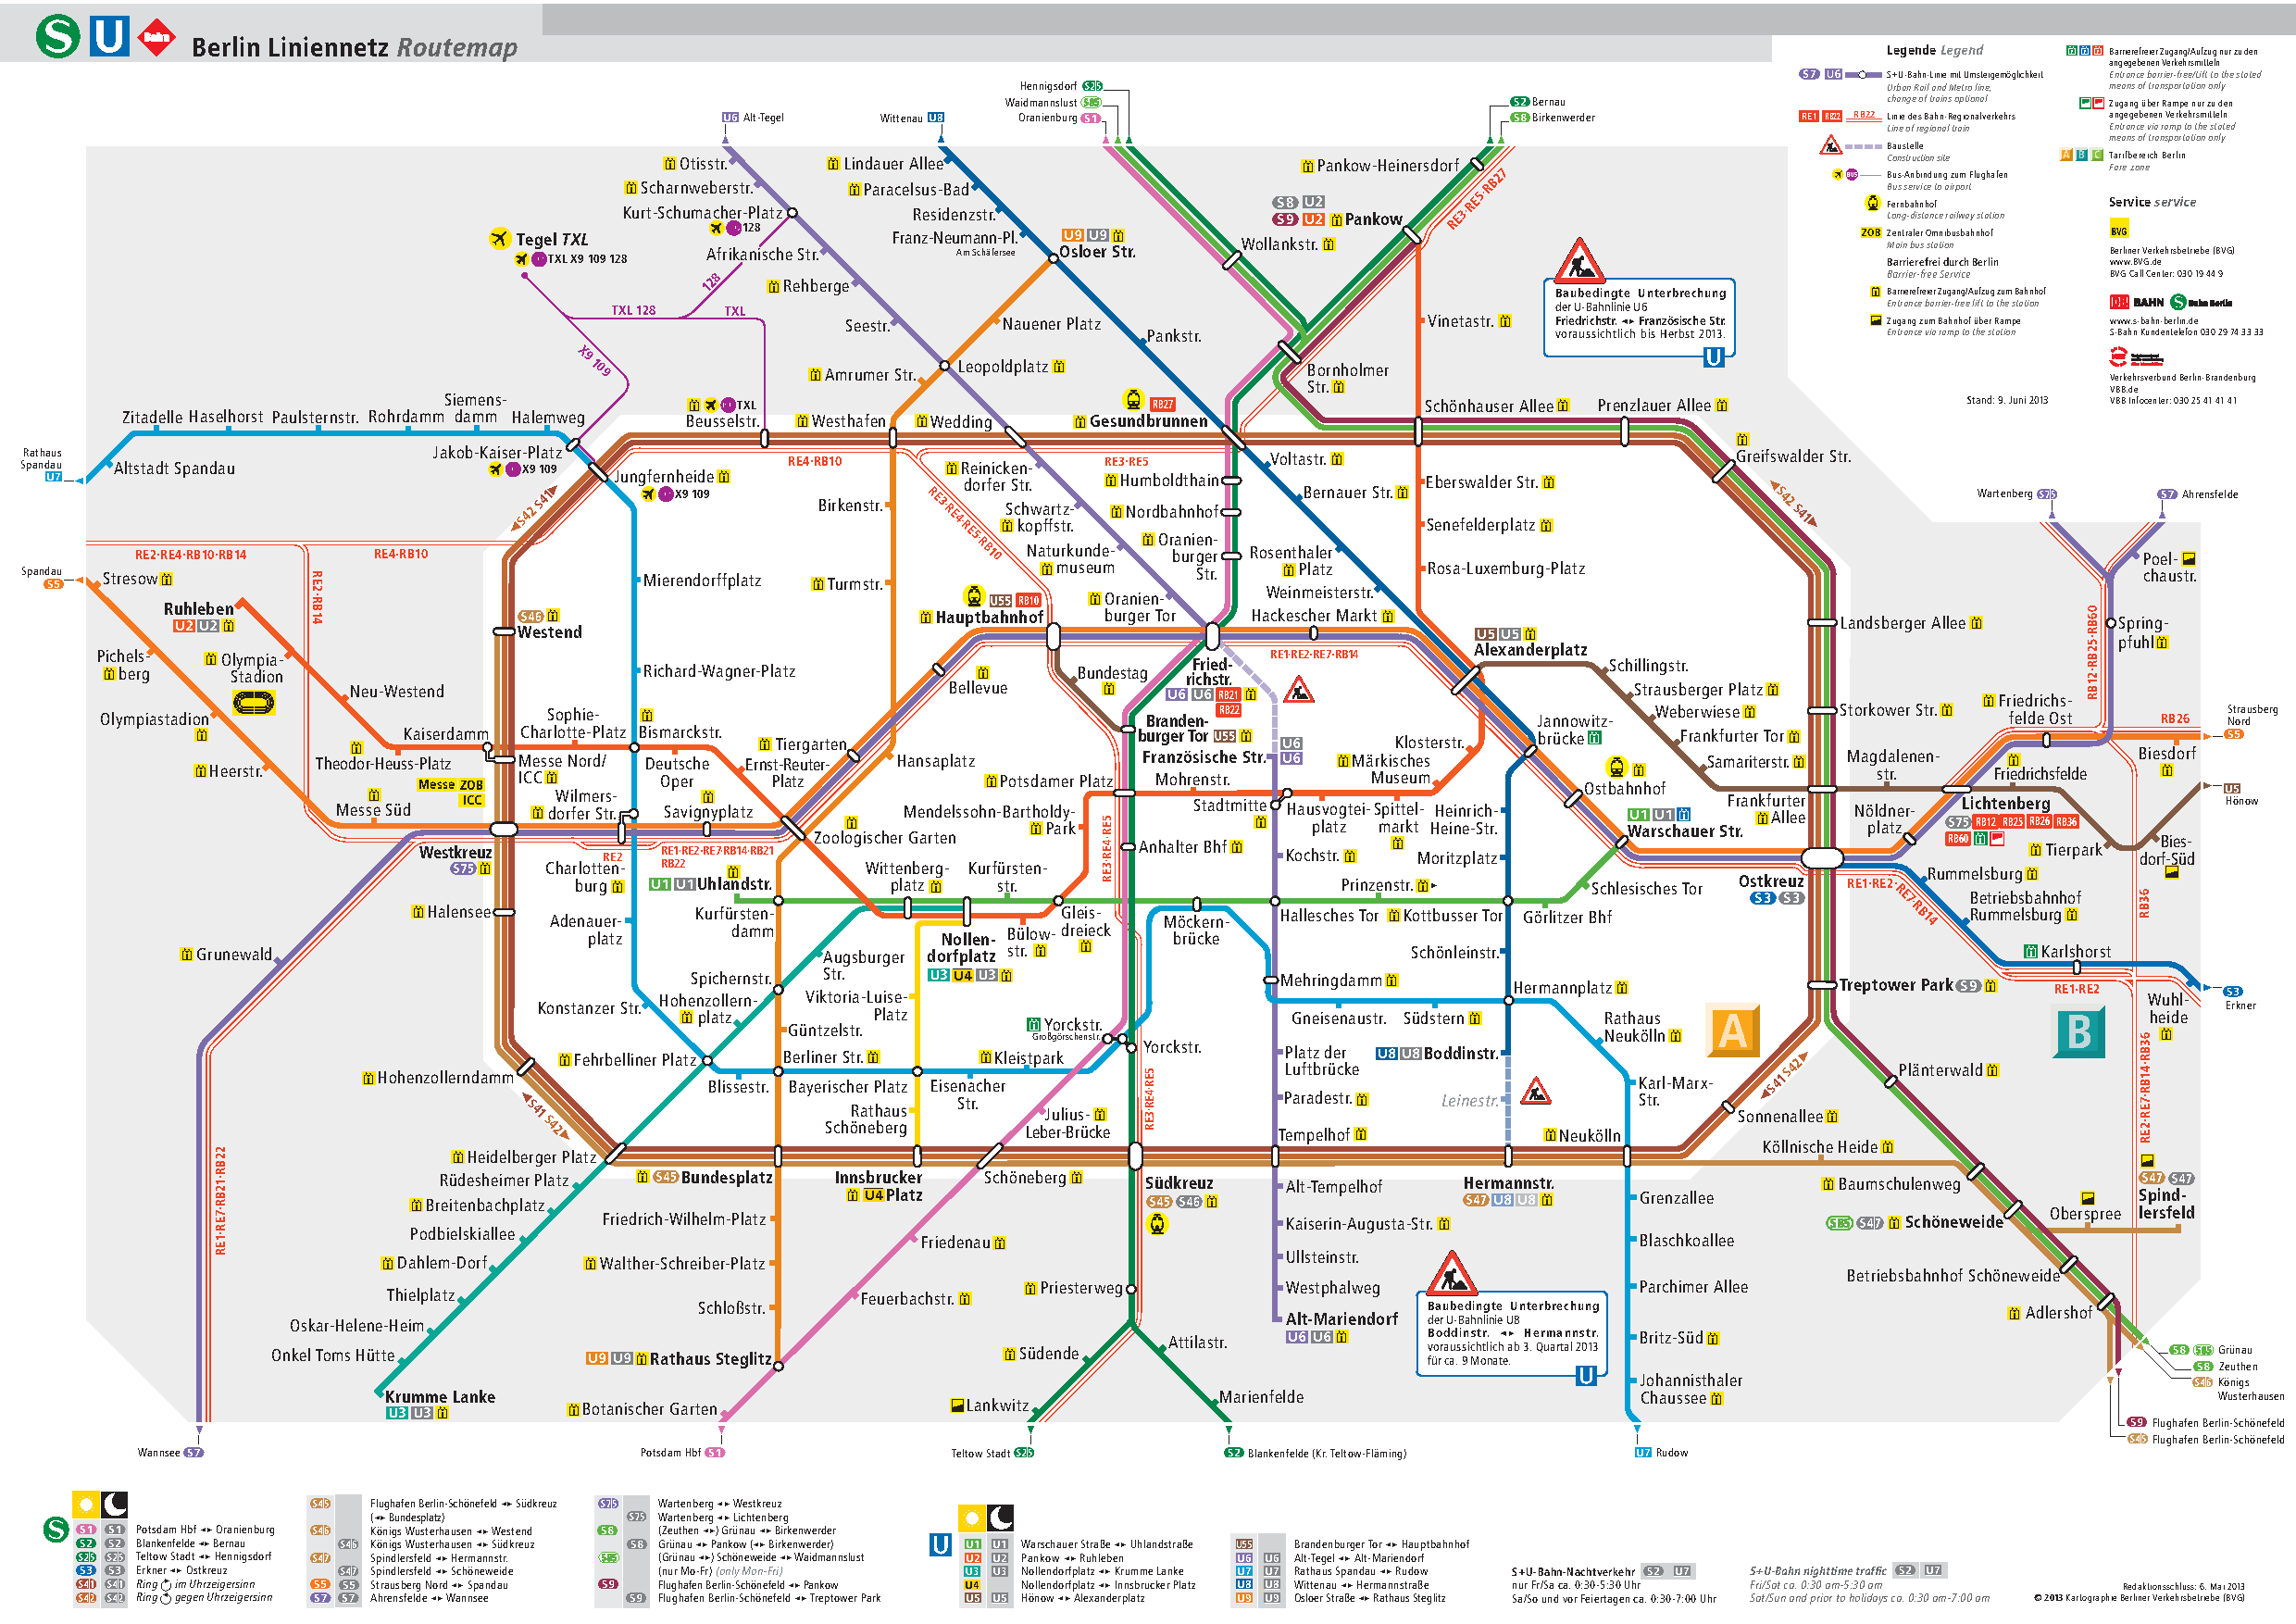
\includegraphics[height=0.9\textwidth, keepaspectratio]{local_img/maps/bvg}
%\end{figure}
%\end{landscape}


%set back fbox frame
\setlength\fboxrule{0pt}

